%!TEX root = ../main.tex 

\section{Comment protéger une alimentation?}

\subsection{Protection antistatique}

\begin{frame}{Décharge Électrostatique (ESD)}
    \begin{columns}
        \begin{column}{0.66\textwidth}
            \begin{itemize}
                \item Norme IEC-61000-4-2
                \begin{itemize}
                    \item Types de décharges
                    \item Méthodologies de tests \& certification
                    \item 4 catégories de produits
                    \item Jusqu'à $\SI{\pm 8}{\kilo\volt}$ / $\SI{\pm 15}{\kilo\volt}$
                \end{itemize}
                \item Deux types de chocs statiques
                \begin{itemize}
                    \item \textbf{Contact Discharge} - Toucher directement chaque pin avec un ESD gun
                    \item \textbf{Air Discharge} - ESD gun proche du DUT jusqu'à décharge
                \end{itemize}
            \end{itemize}
        \end{column}

        \begin{column}{0.33\textwidth}
            \begin{figure}
                \centering
                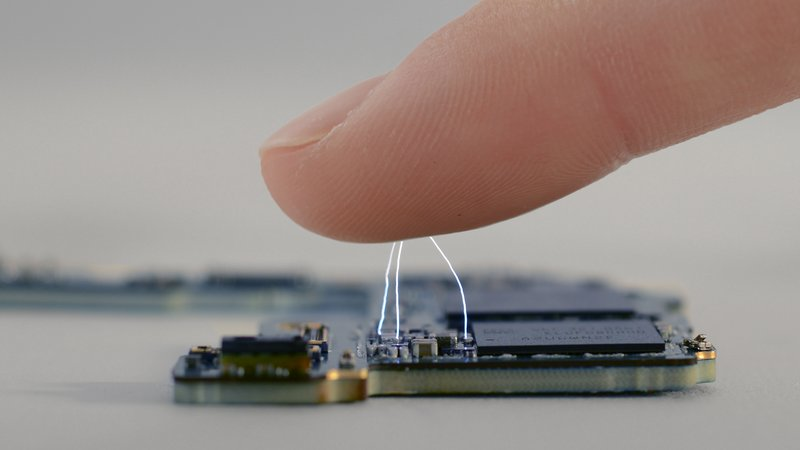
\includegraphics[width=\textwidth]{pictures/ESD-discharge-finger.png}
            \end{figure}
            \begin{figure}
                \centering
                
\includegraphics[width=0.5\textwidth]{pictures/ESD-logo.png}
            \end{figure}
        \end{column}
    \end{columns}
\end{frame}

\begin{frame}{Décharge Électrostatique - Waveform}
    \begin{columns}
        \begin{column}{0.5\textwidth}
        \end{column}
        \begin{column}{0.5\textwidth}
            \begin{itemize}
                \item Pic de courant initial
                \begin{itemize}
                    \item Rise time $\lesssim \SI{1}{\nano\second}$
                \end{itemize}
                \item $2^e$ pic
                \item Chute graduelle
            \end{itemize}
        \end{column}
    \end{columns}

    \vspace{-66pt}

    \begin{figure}
        \centering
        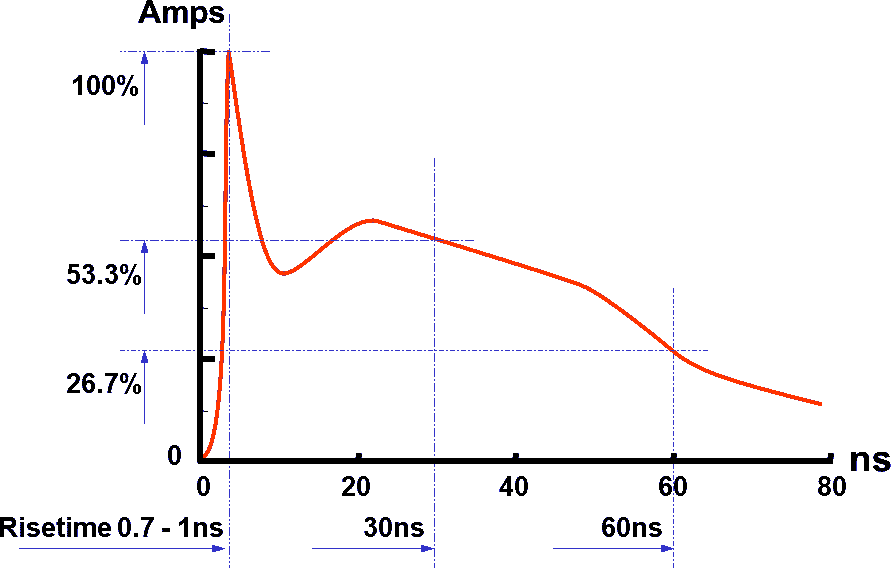
\includegraphics[width=\textwidth]{pictures/ESD-discharge-waveform.png}
    \end{figure}
\end{frame}

\begin{frame}{Circuit protégé antistatiquement - Zener}
    \begin{center}
    \vspace{-24pt}
    \resizebox{\textwidth}{!}{
    \begin{circuitikz}[american voltages]
        \draw [thick]
        (0,-3) to [short, *-] (10,-3)
        to [european resistor, l_=${LOAD}$] (10,1)
        (0,-3) to [open, v<=$V$] (0,1)
        to [short] (10,1)
        ;

        \draw [thick]
        (3, -3) to [empty ZZener diode, color=red] (3, 1);

        % Current spike as a waveform
        \draw[thick, ->] (-0.1, 2) -- (0,3) % Rising edge
        -- (0,3) -- (0.1,1.8) % First sharp drop
        -- (0.2,2.5) -- (0.3,1.9) % Second spike
        -- (0.4,2.3) -- (0.5,2.0) % Smaller oscillation
        -- (0.6,2.15) -- (0.7,2.05) % Final damping
        -- (1,2.1); % Settling

        \node[right] at (1,2.1) {$i_{\text{ESD}}(t) \rightarrow \SI{8}{\kilo\volt}$};
    \end{circuitikz}
    }
    \end{center}
\end{frame}

\begin{frame}{Diode Normale - IV Curve}
    \begin{figure}
        \centering
        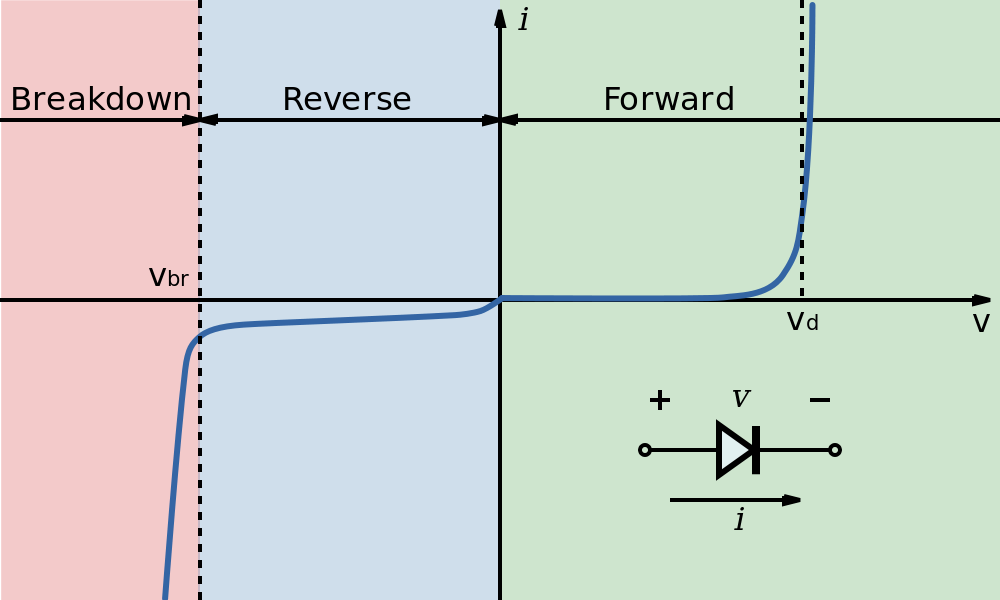
\includegraphics[width=\textwidth]{pictures/diode-iv-curve.png}
    \end{figure}
\end{frame}

\begin{frame}{Diode Zener}
    \begin{columns}
        \begin{column}{0.4\textwidth}
            \begin{itemize}
                \item \textbf{Faite pour être mise à l'envers!}
                \bigskip
                \item $V_Z$ contrôlé
                \item Beaucoup de courant en avalanche
                \item N'endommage pas la diode
                \bigskip
                \item Utilisé dans des références de tension
                \item Utilise comme protection antistatique
            \end{itemize}
        \end{column}
        \begin{column}{0.6\textwidth}
            \begin{figure}
                \centering
                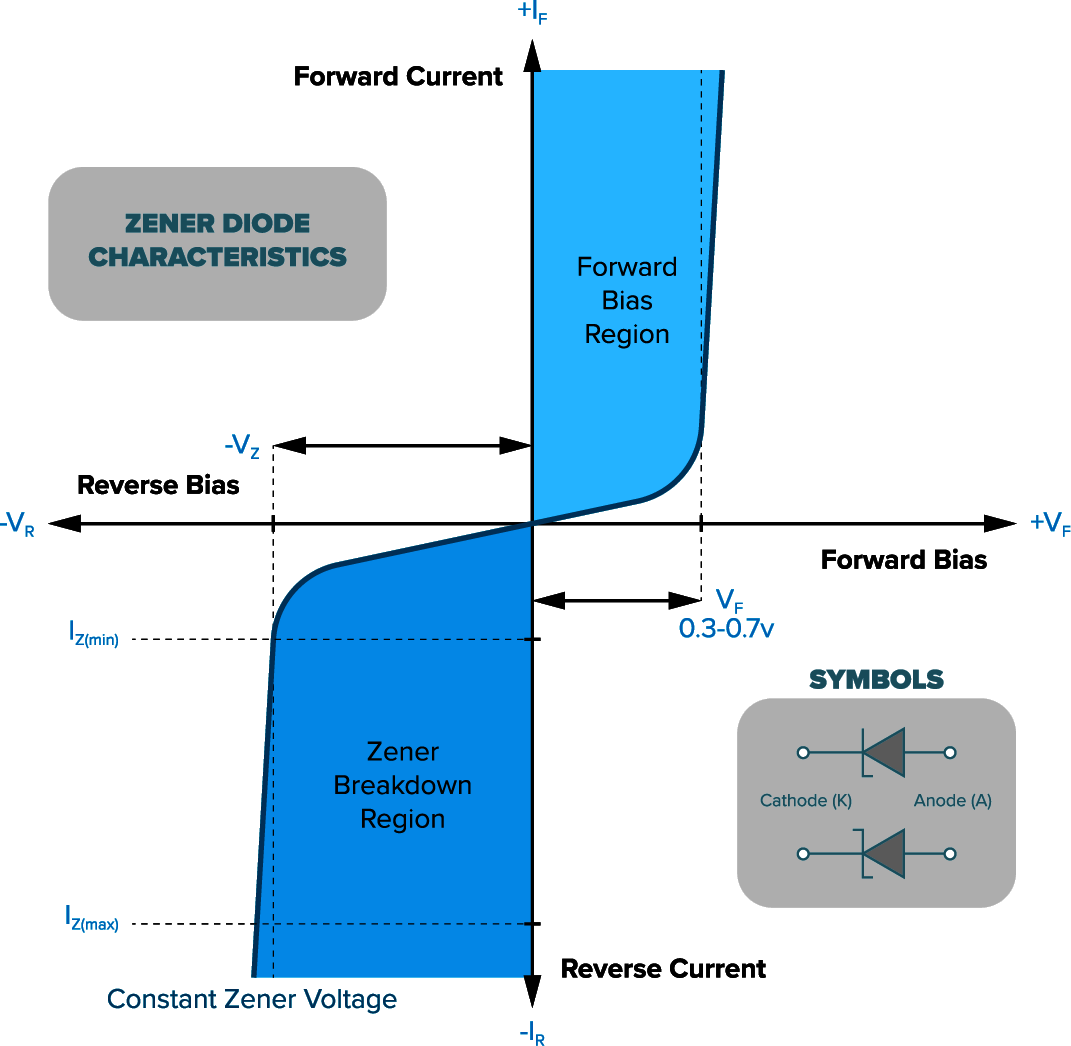
\includegraphics[width=\textwidth]{pictures/diode-zener-iv-curve.png}
            \end{figure}
        \end{column}
    \end{columns}
\end{frame}

\begin{frame}{Circuit protégé antistatiquement}
    \begin{center}
    \vspace{-24pt}
    \resizebox{\textwidth}{!}{
    \begin{circuitikz}[american voltages]
        \draw [thick]
        (0,-3) to [short, *-] (10,-3)
        to [european resistor, l_=${LOAD}$] (10,1)
        (0,-3) to [open, v<=$V$] (0,1)
        to [short] (10,1)
        ;

        \draw [thick]
        (3, -3) to [full ZZener diode, a=$\SI{15}{\volt}$] (3, 1);

        \draw[->, thick, red] 
        (1, 0.75) to[out=0, in=90] (2.75, -0.5);

        % Current spike as a waveform
        \draw[thick, ->]
           (-0.1, 2) -- (0,3)       % Rising edge
        -- (0,3) -- (0.1,1.8)       % First sharp drop
        -- (0.2,2.5) -- (0.3,1.9)   % Second spike
        -- (0.4,2.3) -- (0.5,2.0)   % Smaller oscillation
        -- (0.6,2.15) -- (0.7,2.05) % Final damping
        -- (1,2.1);                 % Settling

        \node[right] at (1,2.1) {$i_{\text{ESD}}(t) \rightarrow \SI{8}{\kilo\volt}$};
    \end{circuitikz}
    }
    \end{center}
\end{frame}


\begin{frame}{Protection avec une diode Zener}
    \begin{itemize}
        \item Clamp le pulse à $V_Z$
        \item Protège les dispositifs par apprès
        \bigskip
        \item Pas l'option la plus rapide
        \item Ne protège pas contre un pulse négatif 
    \end{itemize}

    \begin{figure}
        \centering
        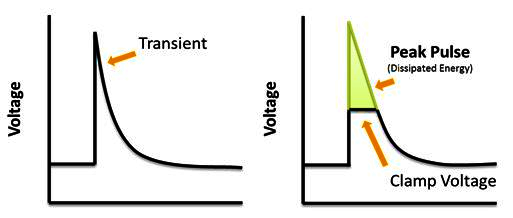
\includegraphics[width=\textwidth]{pictures/clamping-esd-pulse.png}
    \end{figure}
\end{frame}


\begin{frame}{Circuit protégé antistatiquement - TVS}
    \begin{center}
    \vspace{-24pt}
    \resizebox{\textwidth}{!}{
    \begin{circuitikz}[american voltages]
        \draw [thick]
        (0,-3) to [short, *-] (10,-3)
        to [european resistor, l_=${LOAD}$] (10,1)
        (0,-3) to [open, v<=$V$] (0,1)
        to [short] (10,1)
        ;

        % TODO : MODIFIER LA DIODE POUR UNE TVS

        \draw [thick]
        (3, -3) to [empty ZZener diode, color=red] (3, 1);

        % Current spike as a waveform
        \draw[thick, ->] (-0.1, 2) -- (0,3) % Rising edge
        -- (0,3) -- (0.1,1.8) % First sharp drop
        -- (0.2,2.5) -- (0.3,1.9) % Second spike
        -- (0.4,2.3) -- (0.5,2.0) % Smaller oscillation
        -- (0.6,2.15) -- (0.7,2.05) % Final damping
        -- (1,2.1); % Settling

        \node[right] at (1,2.1) {$i_{\text{ESD}}(t) \rightarrow \pm\SI{8}{\kilo\volt}$};

        \draw[->, thick, red] 
        (1, 0.75) to[out=0, in=90] (2.75, -0.5);

        \draw[->, thick, blue] 
        (1, -2.75) to[out=0, in=-90] (2.75, -1.5);
    \end{circuitikz}
    }
    \end{center}
\end{frame}

\begin{frame}{Diode TVS (Transient Voltage Suppression)}
    \begin{columns}
        \begin{column}{0.5\textwidth}
            \begin{itemize}
                \item \textbf{Faite pour protection antistatique!}
                \item \textbf{Bidirectionnel!!}
            \end{itemize}
        \end{column}
        \begin{column}{0.5\textwidth}
            \begin{itemize}
                \item Deux diodes Zener qui se font face
                \item \textit{iv curve} symmétrique
            \end{itemize}
        \end{column}
    \end{columns}
    \begin{figure}
                \centering
                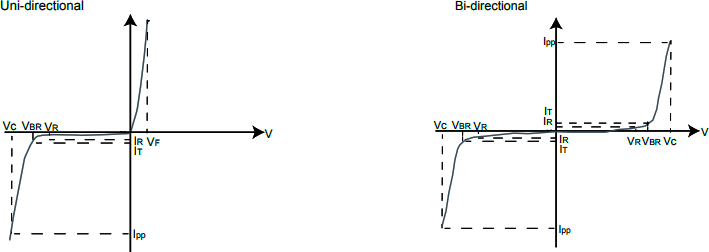
\includegraphics[width=\textwidth]{pictures/diode-tvs-iv-curve.png}
            \end{figure}
\end{frame}

\begin{frame}{Circuit protégé antistatiquement - Condensateur}
    \begin{center}
    \vspace{-24pt}
    \resizebox{\textwidth}{!}{
    \begin{circuitikz}[american voltages]
        \draw [thick]
        (0,-3) to [short, *-] (10,-3)
        to [european resistor, l_=${LOAD}$] (10,1)
        (0,-3) to [open, v<=$V$] (0,1)
        to [short] (10,1)
        ;

        \draw [thick]
        (3, -3) to [C, color=red] (3, 1);

        % Current spike as a waveform
        \draw[thick, ->] (-0.1, 2) -- (0,3) % Rising edge
        -- (0,3) -- (0.1,1.8) % First sharp drop
        -- (0.2,2.5) -- (0.3,1.9) % Second spike
        -- (0.4,2.3) -- (0.5,2.0) % Smaller oscillation
        -- (0.6,2.15) -- (0.7,2.05) % Final damping
        -- (1,2.1); % Settling

        \node[right] at (1,2.1) {$i_{\text{ESD}}(t) \rightarrow \pm\SI{8}{\kilo\volt}$};
    \end{circuitikz}
    }
    \end{center}
\end{frame}


\subsection{Protection de tension inverse}
\begin{frame}{Circuit de protection inverse - Diode}
    \begin{columns}
        \begin{column}{0.33\textwidth}
            \begin{itemize}
                \item Ne conduit que dans un sens
                \bigskip
                \item Drop de tension $V_f$
                \item $P = I \cdot V_f$
            \end{itemize}
        \end{column}
        \begin{column}{0.66\textwidth}
            \begin{center}
            \vspace{-24pt}
            \resizebox{\textwidth}{!}{
            \begin{circuitikz}[american voltages]
                \draw [thick]
                (0, 0) to [short, *-] (10, 0)
                to [european resistor, l_=${LOAD}$] (10, 5)
                (0, 0) to [open, v<=$V$] (0, 5)
                to [short] (4, 5)
                to [empty diode, color=red] (6, 5)
                to [short] (10, 5)
                ;
            \end{circuitikz}
            }
            \end{center}
        \end{column}
    \end{columns}
\end{frame}

\begin{frame}{Circuit de protection inverse - Diode Schottky}
    \begin{columns}
        \begin{column}{0.33\textwidth}
            \begin{itemize}
                \item Ne conduit que dans un sens
                \bigskip
                \item Drop de tension $V_f$ plus petite
                \item $P = I \cdot V_f$
                \bigskip
                \item Plus cher pour même rating de courant
            \end{itemize}
        \end{column}
        \begin{column}{0.66\textwidth}
            \begin{center}
            \vspace{-24pt}
            \resizebox{\textwidth}{!}{
            \begin{circuitikz}[american voltages]
                \draw [thick]
                (0, 0) to [short, *-] (10, 0)
                to [european resistor, l_=${LOAD}$] (10, 5)
                (0, 0) to [open, v<=$V$] (0, 5)
                to [short] (4, 5)
                to [empty Schottky diode, color=red] (6, 5)
                to [short] (10, 5)
                ;
            \end{circuitikz}
            }
            \end{center}
        \end{column}
    \end{columns}
\end{frame}

\begin{frame}{Circuit de protection inverse - PMOS}
    \begin{columns}
        \begin{column}{0.33\textwidth}
            \begin{itemize}
                \item Ne conduit que dans un sens
                \bigskip
                \item Drop de tension vraiment plus petite ($R_{ds_{on}} \cdot I$)
                \bigskip
                \item Tension maximale supportée
            \end{itemize}
        \end{column}
        \begin{column}{0.66\textwidth}
            \begin{center}
            \vspace{-24pt}
            \resizebox{\textwidth}{!}{
            \begin{circuitikz}[american voltages]
                \draw [thick]
                (0, 0) to [short, *-] (10, 0)
                to [european resistor, l_=${LOAD}$] (10, 5)
                (0, 0) to [open, v<=$V$] (0, 5);
                
                \draw   (4,5) node[pigfete, bodydiode, color=red, rotate=90, xscale=2, yscale=-2] (fet) {}
                (fet.G) node [anchor=south, xshift=8pt] {G}
                (fet.D) node [anchor=west, yshift=8pt] {D}
                (fet.S) node [anchor=east, yshift=8pt] {S}
                (fet.G) to [short, -*] (fet.G |- 0,0)
                (fet.D) to [short, -*] (0, 5)
                (fet.S) to (10, 5);
            \end{circuitikz}
            }
            \end{center}
        \end{column}
    \end{columns}
\end{frame}

\begin{frame}{Transistor MOSFET P-Channel (PMOS)}
    \begin{columns}
        \begin{column}{0.75\textwidth}
            \begin{center}
                $V_{gs}$ négatif!\\
                \vspace{6pt}
                $V_{gs} < -V_t$\\
                \vspace{8pt}
                Faire attention au $V_{gs_{max}}$
            \end{center}
            \vspace{24pt}

            \begin{columns}
                \begin{column}{0.5\textwidth}
                    %\textbf{Branchement normal}
                    \begin{itemize}
                        \item $V_G = \SI{0}{\volt}$
                        \item $V_{gs} = -VDD$
                        \item $-VDD < -V_t$
                        \item Conduit!
                    \end{itemize}
                \end{column}
                \begin{column}{0.5\textwidth}
                    %\textbf{Branchement inverse}
                    \begin{itemize}
                        \item $V_G = VDD$
                        \item $V_{gs} = \SI{0}{\volt}$
                        \item $\SI{0}{\volt} > -V_t$
                        \item Ne conduit pas
                    \end{itemize}
                \end{column}
            \end{columns}
        \end{column}

        \begin{column}{0.25\textwidth}
            \begin{center}
            \vspace{-24pt}
            \resizebox{!}{0.75\textheight}{
            \begin{circuitikz}[american voltages]
                
                \draw   (2,0) node[pigfete, bodydiode, xscale=1.5, yscale=1.5] (fet) {}
                (fet.G) node [anchor=east, yshift=8pt] {G}
                (fet.D) node [anchor=south, xshift=8pt, yshift=-4pt] {D}
                (fet.S) node [anchor=north, xshift=8pt, yshift=4pt] {S}
                (fet.G) to [short, -*] (fet.G |- 0, 0.4)
                (fet.D) to [short] (2, 2)
                ++(0,0) node[vcc]{VDD}
                (fet.S) to [short] (2, -1.5)
                to [R] (2, -3.5)
                to (2, -3.75) node[ground]{}
                ;

                \draw[->, thick, red] 
                (1, 0.75) to[out=90, in=180] (1.75, 1.5);

                \node[right] at (0.66, 1.66) {$V_{gs}$};
            \end{circuitikz}
            }
            \end{center}
        \end{column}
    \end{columns}
\end{frame}

\begin{frame}{Circuit de protection inverse - PMOS complèt}
    \begin{columns}
        \begin{column}{0.33\textwidth}
            \begin{itemize}
                \item Ne conduit que dans un sens
                \bigskip
                \item Drop de tension vraiment plus petite ($R_{ds_{on}} \cdot I$)
                \bigskip
                \item Supporte toutes les tensions!
            \end{itemize}
        \end{column}
        \begin{column}{0.66\textwidth}
            \begin{center}
            \vspace{-24pt}
            \resizebox{\textwidth}{!}{
            \begin{circuitikz}[american voltages]
                \draw [thick]
                (0, 0) to [short, *-] (10, 0)
                to [european resistor, l_=${LOAD}$] (10, 5)
                (0, 0) to [open, v<=$V$] (0, 5);
                
                \draw   (4,5) node[pigfete, bodydiode, color=red, rotate=90, xscale=2, yscale=-2] (fet) {}
                (fet.G) node [anchor=south, xshift=8pt] {G}
                (fet.D) node [anchor=west, yshift=8pt] {D}
                (fet.S) node [anchor=east, yshift=8pt] {S}
                (fet.G) to [R] (fet.G |- 0,0)
                (fet.D) to [short, -*] (0, 5)
                (fet.S) to (10, 5)
                (fet.G) to [short] (fet.G -| 6,3)
                to [full ZZener diode] (6, 5);
            \end{circuitikz}
            }
            \end{center}
        \end{column}
    \end{columns}
\end{frame}


\subsection{Protection de court-circuit}

\subsection{Protection de inrush current}
\subsection{GFCI \& Grounding}